\section{Mini-jeux}

\subsection{Jeu des carrés d'aires}
\begin{multicols}{2}
    \boite{Règles : }{
        \begin{enumerate}
            \item On lance deux dés et on dessine un rectangle aux dimensions correspondantes. 
            \item Le premier joueur commence dans un coin et l'adversaire dans celui opposé. 
            \item Tous les rectangles d'un joueur doivent être connectés. 
            \item On ne peut pas chevaucher un rectangle, allié ou adverse. 
            \item Si tu ne peux pas jouer, tu passes ton tour. 
            \item Quand il n'y a pas plus d'espace libre, la partie s'arrête. 
            \item Un rectangle rapporte un nombre de points égal au produit des deux dés.
            \item Celui qui a le plus de points l'emporte.
        \end{enumerate}
    }
    
    \columnbreak

    \begin{center}
        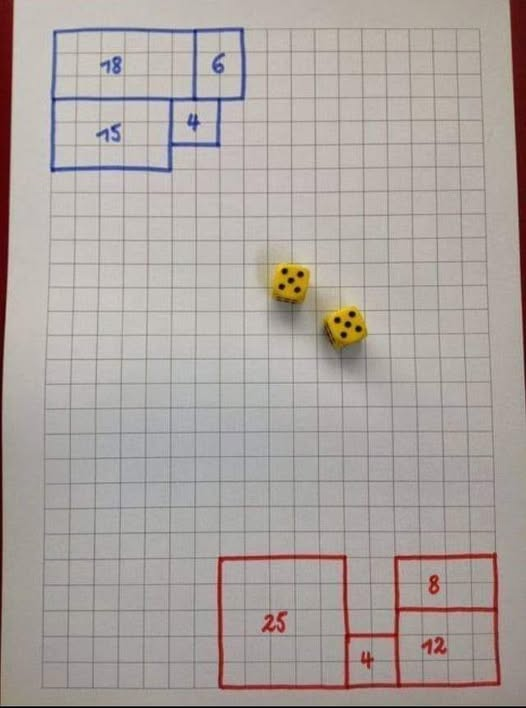
\includegraphics[width=0.45\textwidth]{images/jeu_carre_aire.jpg}
    \end{center}
\end{multicols}

\vspace{-0.7cm}\subsection{Juniper Green}


\begin{Definition}[Multiple et diviseur]
    \vspace{-0.2cm}\begin{multicols}{2}
    On dit qu'un nombre entier est \acc{multiple} d'un autre nombre entier si le premier nombre est dans la \acc{table de multiplication} du second. \\
       
    \columnbreak

    \textbf{Exemple : }

    $12$ est un \acc{multiple} de $3$ car $12 = 4 \times 3$.
\end{multicols}

    \vspace{-0.75cm}\begin{multicols}{2}
        On dit qu'un nombre entier est un \acc{diviseur} d'un autre nombre entier si on peut \acc{effectuer} la \acc{division} du second nombre par le premier, avec un \acc{reste} nul.  

        \columnbreak

        \textbf{Exemple : }

        $5$ est un \acc{diviseur} de $20$ car \opidiv{20}{5}

        Le reste vaut $0$.
    \end{multicols}
\end{Definition}
\vspace{-0.25cm}\begin{multicols}{2}
\boite{Matériel :}{
\begin{itemize}[itemsep=0em]
    \item Un plateau de jeu composé de : \textbf{un tableau de jeu} et d'\textbf{une pochette plastique}.
    \item Des feutres effaçables.
    \item Une feuille de brouillon
\end{itemize}
}

\columnbreak

\boite{Règles du jeu}{
\begin{itemize}[itemsep=0em]
    \item Le joueur qui commence barre un nombre pair.
    \item Ensuite, chaque joueur, à tour de rôle, barre un nombre parmi les \textbf{multiples} ou les \textbf{diviseurs} du nombre barré par son adversaire.
\end{itemize}
}
\end{multicols}
\vspace{-0.5cm}\boite{Objectif : }{
    \textbf{Un joueur est déclaré gagnant lorsque son adversaire ne peut plus jouer.}
}

%\newpage 

\boite{Exemple de tour de jeu :}{
\begin{itemize}
    \item Si le joueur A barre le 12, le joueur B doit barrer un multiple ou un diviseur de 12. Il n'y a pas de multiple de 12 sur le plateau, il a donc le choix entre les diviseurs de 12 : 1 ; 2 ; 3 ; 4 et 6. Supposons que le joueur B barre le 3.
    \item Le joueur A peut alors barrer le 1, le 6, le 9, le 15 ou le 18. Supposons qu'il barre le 9.
    \item Le joueur B ne peut plus barrer que le 1 ou le 18. Supposons qu'il barre le 1.
    \item Le joueur A peut alors barrer n'importe quel nombre restant sur le plateau. Supposons qu'il barre le 19. Le joueur B ne peut plus jouer. Le joueur A est déclaré gagnant.
\end{itemize}
}

%\vspace{-1cm}\section*{Plateaux de jeux}

\begin{multicols}{2}
\boite{Niveau 1 :}{\begin{center}
\begin{tabular}{|c|c|c|c|c|}
\hline
1 & 2 & 3 & 4 \\
\hline
5 & 6 & 7 & 8 \\
\hline
9 & 10 & 11 & 12 \\
\hline
13 & 14 & 15 & 16 \\
\hline
17 & 18 & 19 & 20 \\
\hline
\end{tabular}
\end{center}
}
\boite{Niveau 2 :}{
\begin{center}
\begin{tabular}{|c|c|c|c|c|}
\hline
1 & 2 & 3 & 4 & 5 \\
\hline
6 & 7 & 8 & 9 & 10 \\
\hline
11 & 12 & 13 & 14 & 15 \\
\hline
16 & 17 & 18 & 19 & 20 \\
\hline
21 & 22 & 23 & 24 & 25 \\
\hline
26 & 27 & 28 & 29 & 30 \\
\hline
31 & 32 & 33 & 34 & 35 \\
\hline
36 & 37 & 38 & 39 & 40 \\
\hline
\end{tabular}
\end{center}
}

\columnbreak

\boite{Niveau 3 :}{
\begin{center}
\begin{tabular}{|c|c|c|c|c|c|c|c|c|c|}
\hline
1 & 2 & 3 & 4 & 5 & 6 & 7 & 8 & 9 & 10 \\
\hline
11 & 12 & 13 & 14 & 15 & 16 & 17 & 18 & 19 & 20 \\
\hline
21 & 22 & 23 & 24 & 25 & 26 & 27 & 28 & 29 & 30 \\
\hline
31 & 32 & 33 & 34 & 35 & 36 & 37 & 38 & 39 & 40 \\
\hline
41 & 42 & 43 & 44 & 45 & 46 & 47 & 48 & 49 & 50 \\
\hline
51 & 52 & 53 & 54 & 55 & 56 & 57 & 58 & 59 & 60 \\
\hline
61 & 62 & 63 & 64 & 65 & 66 & 67 & 68 & 69 & 70 \\
\hline
71 & 72 & 73 & 74 & 75 & 76 & 77 & 78 & 79 & 80 \\
\hline
81 & 82 & 83 & 84 & 85 & 86 & 87 & 88 & 89 & 90 \\
\hline
91 & 92 & 93 & 94 & 95 & 96 & 97 & 98 & 99 & 100 \\
\hline
\end{tabular}
\end{center}
}
\end{multicols} % Inclusion de l'énoncé

\newpage 

\subsection{Multiplicato}

\begin{multicols}{2}
\boite{Matériel :}{
\begin{itemize}
    \item La feuille de jeu
    \item Un stylo rouge
    \item Un stylo bleu
\end{itemize}
}

\columnbreak

\boite{But :}{
Faire le plus possible d'alignements d'au moins trois nombres en ligne ou en colonne, contigus ou non, en les entourant de sa couleur.
}
\end{multicols}

\begin{multicols}{2}
\boite{Nombre de joueurs :}{
2 joueurs.
}

\columnbreak

\boite{Mécanisme :}{
Un coup est valide quand le joueur annonce un produit égal au nombre qu'il a choisi sur la grille. Les produits doivent se situer dans la limite de 10 x 10 pour le niveau 1 et de 12 x 12 pour le niveau 2.\\

Lien vers la démo : \href{https://jeux2maths.fr/multiplicato/}{https://jeux2maths.fr/multiplicato/}
}
\end{multicols}

\begin{multicols}{2}
\boite{Déroulement d'une partie :}{
\begin{itemize}
    \item Un joueur se munit d'un stylo rouge, l'autre d'un stylo bleu. La feuille de jeu est placée entre les joueurs.
    \item L'adversaire impose au joueur de choisir un nombre dans une table de multiplication pour laquelle il existe un produit disponible sur la grille.
    \item Le joueur annonce le produit correspondant au nombre qu'il choisit sur la grille, entoure ce nombre lorsque son adversaire a validé le choix et écrit le produit dans sa colonne sur la feuille de jeu. Il impose à son tour une table de multiplication dans laquelle son adversaire devra jouer.
    \item Si l'adversaire propose une table pour laquelle il n'existe plus de nombre disponible sur la grille, le joueur entoure un nombre de son choix.
    \item Si le joueur commet une erreur dans son produit, il ne peut jouer, et c'est alors l'adversaire qui entoure un nombre de son choix.
    \item La partie se termine quand tous les nombres sont entourés sur la grille.
\end{itemize}
}

\columnbreak

\boite{Scores :}{
Les points sont comptés à l'issue de la partie.
\begin{itemize}
    \item Un alignement de 3 nombres dans une couleur vaut 1 point.
    \item Un alignement de 4 nombres dans une couleur vaut 3 points.
    \item Un alignement de 5 nombres dans une couleur vaut 10 points.
\end{itemize}
Le vainqueur est le joueur qui totalise le plus de points à l'issue de la partie.

Remarque : on peut également comptabiliser les alignements effectués en diagonale, mais le comptage s'avère alors difficile pour la majeure partie des élèves.
}
\end{multicols} % Inclusion de la solution

